\documentclass[10pt]{article}
\usepackage[margin=0.85in]{geometry}
\usepackage{graphicx}
\usepackage{amsmath}
\usepackage{booktabs}
\usepackage{siunitx}
\usepackage[font=small,labelfont=bf,skip=3pt]{caption}
\usepackage{xcolor}
\usepackage[colorlinks=true,linkcolor=blue!50!black,citecolor=blue!50!black]{hyperref}

% Compact section spacing (avoids the titlesec dependency)
\makeatletter
\renewcommand\section{\@startsection{section}{1}{\z@}%
  {-1.2ex \@plus -0.4ex \@minus -0.2ex}{0.5ex \@plus 0.2ex}%
  {\normalfont\large\bfseries}}
\makeatother

\graphicspath{{figures/}}
\setlength{\parskip}{3pt}
\setlength{\parindent}{0pt}
\captionsetup{belowskip=2pt}

\title{\vspace{-1.5em}\textbf{How many clusters? A 5-state vs.\ 7-state comparison\\of the VAE--HMM convection model}}
\author{Complementary report}
\date{\today}

\begin{document}
\maketitle
\vspace{-2em}

\section{Motivation}

The paper analyses convective organization through a VAE--HMM with $K=7$ latent
states. A natural question is whether the headline results---(i) a
precipitation/organization plane of variability, (ii) an organized, high-PW
cluster with deep coherent mass flux, (iii) a two-regime leading non-stationary
mode~$v_2$, and (iv) residual non-Markovian memory in the organized
cluster---are genuine physical features or artifacts of the chosen cluster count.
We refit the analysis on a $K=5$ model (\texttt{exp\_20260223\_1140\_5c129e};
identical VAE backbone, \texttt{latent\_dim}=8, \texttt{hidden\_dim}=512) and
compare it to the $K=7$ paper model state by state. Both models are applied to the
same \num{19475}-step time series, so clusters can be mapped directly through their
temporal co-occurrence.

\section{Cluster structure and 7\,$\rightarrow$\,5 mapping}

\begin{figure}[htbp]
\centering
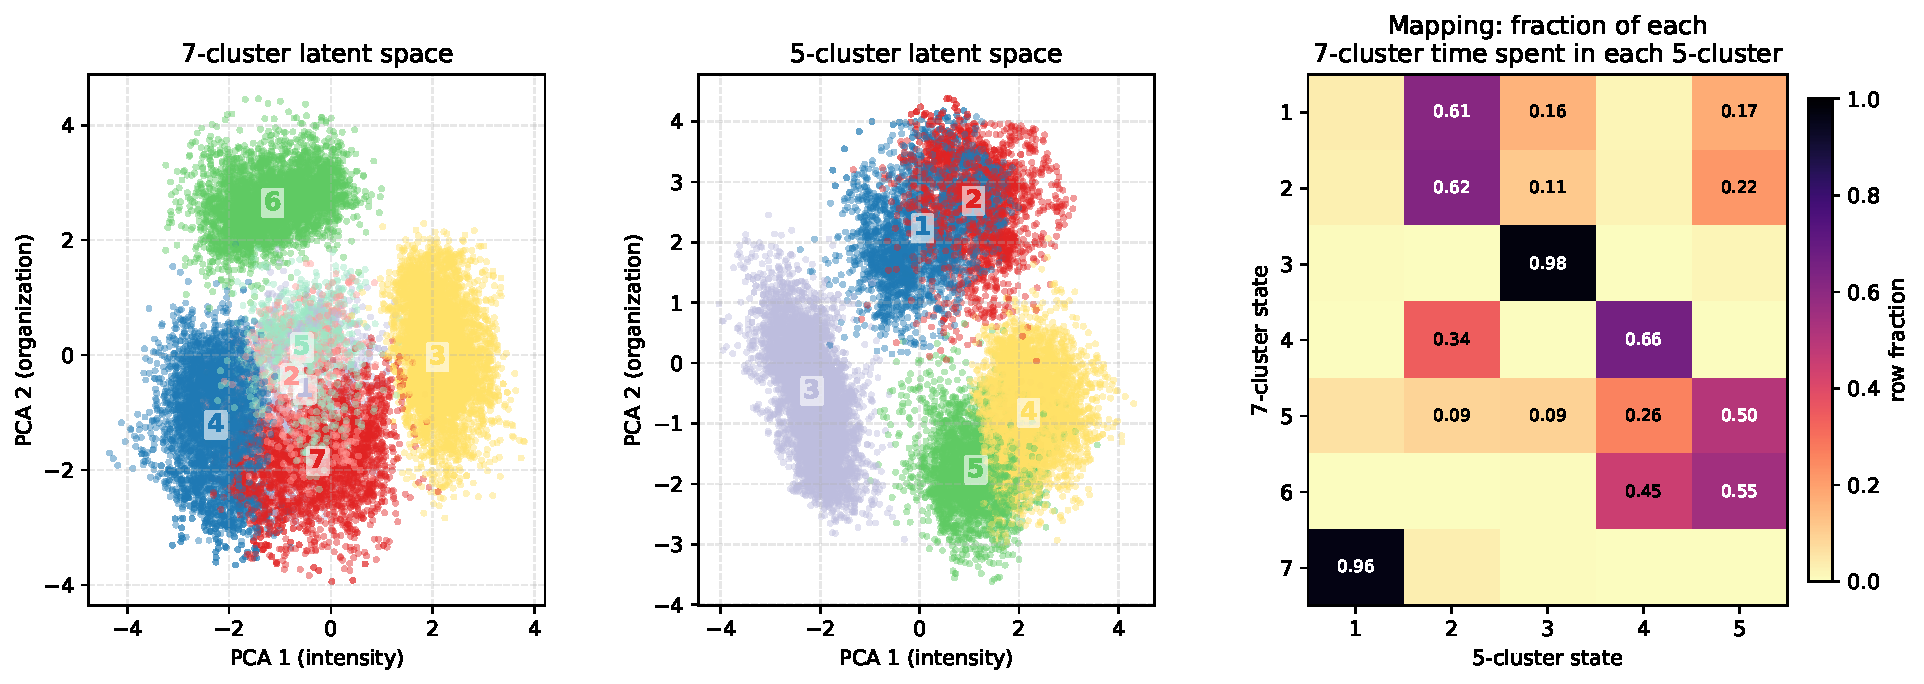
\includegraphics[width=0.9\textwidth]{fig1_clusters_mapping.pdf}
\caption{Latent PCA space coloured by cluster for the 7-state (left) and 5-state
(middle) models, and the co-occurrence mapping (right): each row is a 7-cluster
state, each column a 5-cluster state, and the cell gives the fraction of that
7-cluster's time that the 5-state model assigns to the corresponding 5-cluster
(rows sum to~1).}
\label{fig:map}
\end{figure}

Both models partition the same latent geometry (Fig.~\ref{fig:map}): a large
quiescent core, a moist/organized lobe at high PC2, and a dry, convectively
active lobe at low PC2. The mapping is highly structured rather than a reshuffle:

\begin{itemize}\setlength{\itemsep}{1pt}
\item \textbf{Two anchor states are preserved almost 1:1.} The organized,
highest-PW cluster (7c\,7, PW\,$=16.9$) maps to 5c\,1 (PW\,$=16.9$) with fraction
$0.96$; the large quiescent cluster (7c\,3) maps to 5c\,3 with fraction $0.98$.
\item \textbf{The moderate-moisture band merges.} 7c\,1 and 7c\,2 (PW\,$\approx$\,9--10,
moderate precip) collapse into a single 5c\,2 ($\approx0.61$--$0.62$ each).
\item \textbf{The dry/active band is redistributed.} The heavy-precip 7c\,4 maps
mostly to 5c\,4 ($0.66$); the high-PC2 active state 7c\,6 splits between 5c\,5
($0.55$) and 5c\,4 ($0.45$); the transitional 7c\,5 goes mainly to 5c\,5.
\end{itemize}

So coarsening from 7 to 5 keeps the physically extreme states (organized,
quiescent) intact and merges the intermediate moisture/activity band. Table~\ref{tab:fp}
lists the per-cluster fingerprints.

\begin{table}[htbp]
\centering
\caption{Per-cluster fingerprints. $n$: occupancy; precip and PW: domain
diagnostics; $\pi$: stationary weight; RMSE: gap between the empirical indicator
autocorrelation and the Markov prediction (larger = more non-Markovian).}
\label{tab:fp}
\small
\begin{tabular}{l r r r r r r}
\toprule
\multicolumn{7}{l}{\textbf{7-cluster model} \quad (PCA EVR $=0.21,0.18$)}\\
\midrule
State & $n$ & precip & PW & $\pi$ & RMSE & note\\
\midrule
1 & 886  & 3.82 & 9.35  & 0.046 & 0.122 & \\
2 & 686  & 4.19 & 10.26 & 0.035 & 0.128 & \\
3 & 7086 & 1.68 & 9.35  & 0.364 & 0.078 & quiescent\\
4 & 3703 & 5.36 & 6.07  & 0.191 & 0.061 & heavy precip\\
5 & 777  & 3.06 & 5.85  & 0.040 & 0.076 & \\
6 & 3819 & 3.06 & 3.55  & 0.197 & \textbf{0.254} & organized/active\\
7 & 2518 & 4.74 & 16.88 & 0.127 & \textbf{0.275} & organized (max PW)\\
\midrule
\multicolumn{7}{l}{\textbf{5-cluster model} \quad (PCA EVR $=0.23,0.18$)}\\
\midrule
State & $n$ & precip & PW & $\pi$ & RMSE & note\\
\midrule
1 & 2562 & 4.69 & 16.85 & 0.129 & \textbf{0.287} & organized (max PW)\\
2 & 2376 & 4.99 & 9.85  & 0.122 & 0.156 & moist, intense precip\\
3 & 7230 & 1.71 & 9.42  & 0.370 & 0.087 & quiescent\\
4 & 4380 & 4.52 & 4.04  & 0.227 & \textbf{0.227} & dry/active\\
5 & 2927 & 2.74 & 4.22  & 0.152 & 0.112 & dry transitional\\
\bottomrule
\end{tabular}
\end{table}

\section{Axes of variability: precipitation and organization}

In both models PC1 tracks intensity and PC2 tracks organization. The Pearson
correlations (signs are arbitrary; magnitudes are comparable) are
$|r(\text{PC1},\text{precip})| = 0.62$ (7c) vs.\ $0.55$ (5c) and
$|r(\text{PC2},\text{PW})| = 0.63$ (7c) vs.\ $0.68$ (5c). The
precipitation/organization plane is therefore \emph{not} an artifact of cluster
count: it is intrinsic to the VAE latent space, which the HMM merely partitions.
If anything the organization (PW) axis is slightly better expressed at $K=5$,
and the explained variance of the first two PCs is essentially unchanged
($0.39$ vs.\ $0.41$).

\section{Vertical structure: positive vs.\ negative mass flux}

\begin{figure}[htbp]
\centering
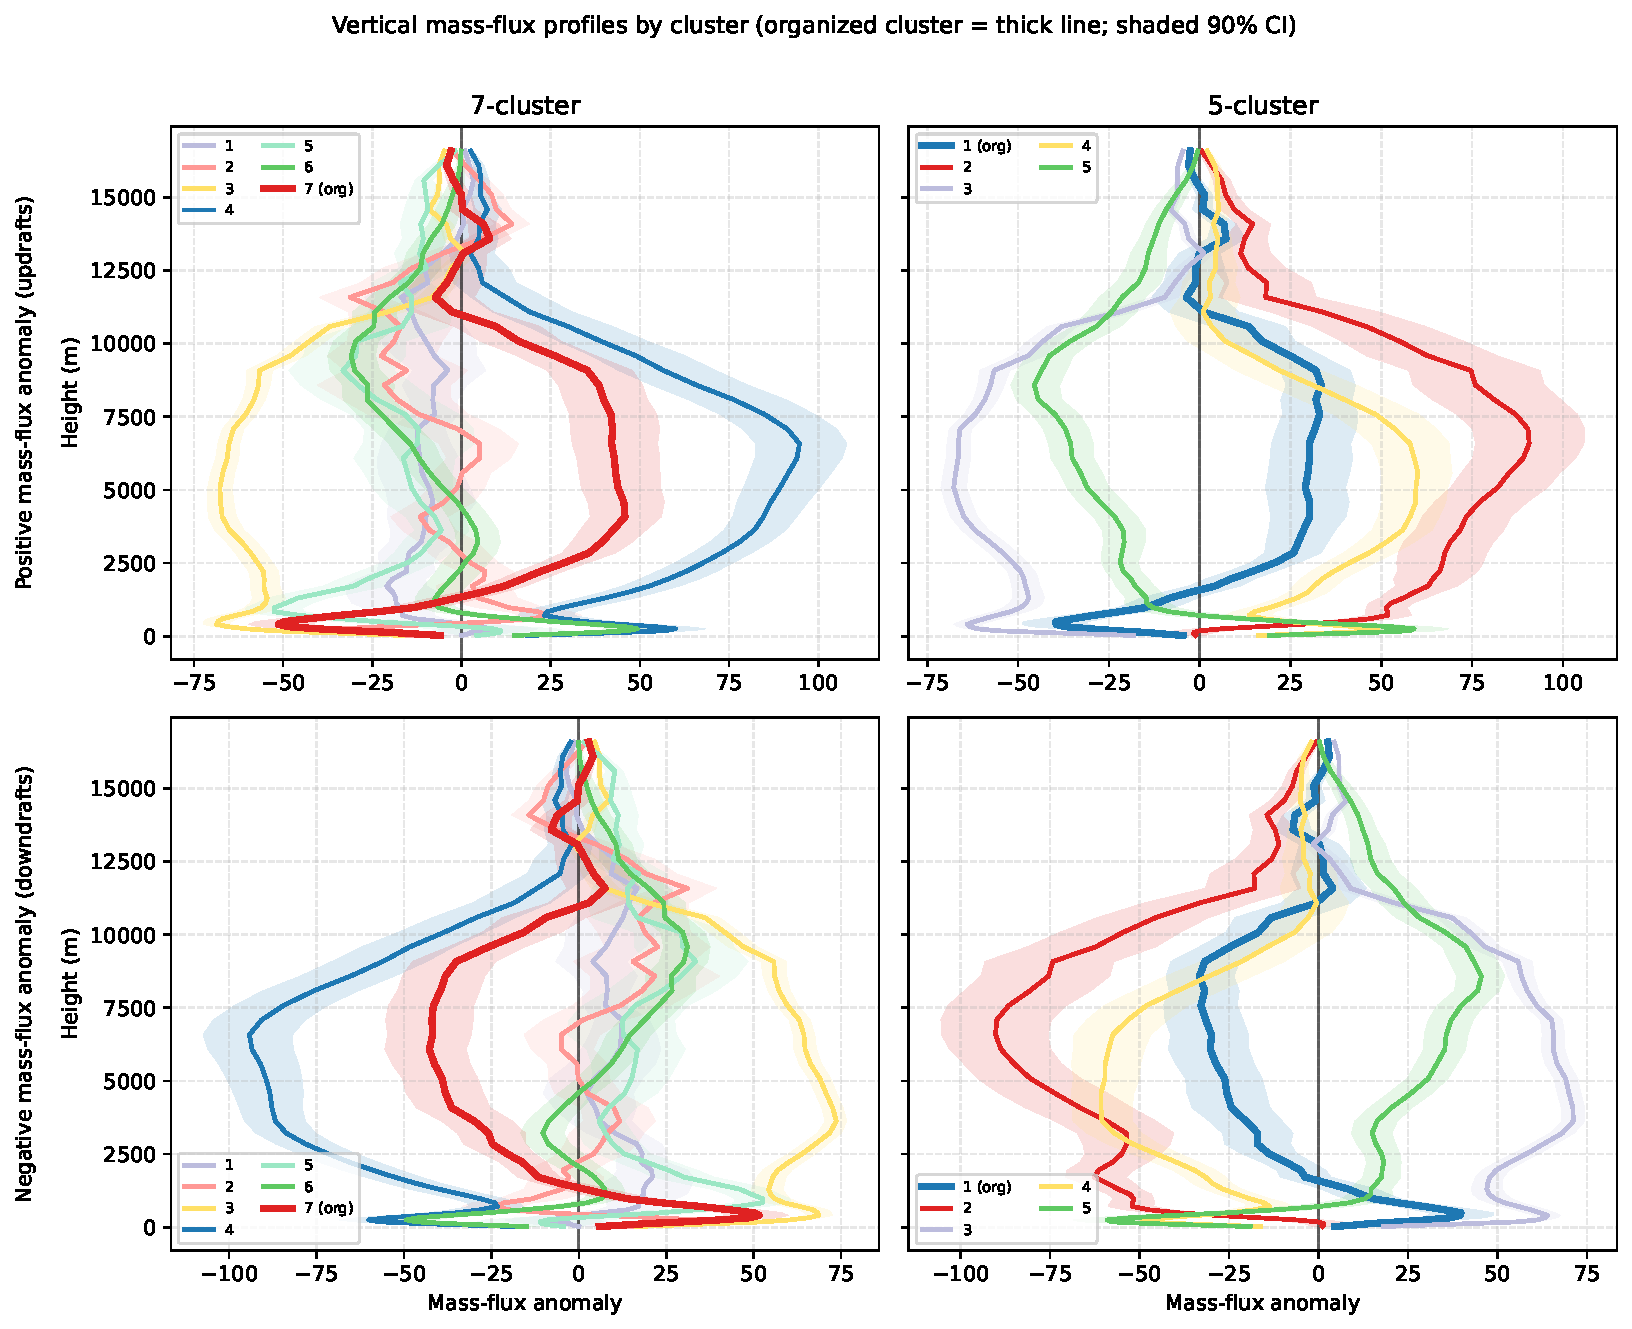
\includegraphics[width=0.6\textwidth]{fig5_massflux_pos_neg.pdf}
\caption{Per-cluster vertical profiles of the positive (top, updrafts) and
negative (bottom, downdrafts) mass-flux anomaly, for the 7-state (left) and
5-state (right) models. Profiles are bootstrap means over the closest-to-centroid
samples (shaded: 90\% CI); the organized (max-PW) cluster is drawn thick.}
\label{fig:mf}
\end{figure}

Decomposing the mass flux into its positive (updraft) and negative (downdraft)
parts shows the same physical ordering of clusters in both models
(Fig.~\ref{fig:mf}). The organized cluster carries a deep, strong updraft anomaly
peaking in the mid-to-upper troposphere ($\sim$8--9~km) together with the largest
compensating downdraft anomaly---the signature of deep, vertically coherent
convection---while the quiescent cluster is near zero at all levels and the
dry/active clusters show shallow, low-level structure. The updraft/downdraft
contrast is therefore not an artifact of cluster count.

The one difference mirrors the mapping (\S2): at $K=7$ the deepest, strongest
updraft belongs to the organized high-PW state 7c\,7, whereas at $K=5$ that
maximal updraft is shared between the organized 5c\,1 and the intense-precip
5c\,2---the two states that absorb 7c\,7 and the moderate-moisture band. The
five-state model thus splits the ``deep convection'' signature across its two
moist clusters rather than concentrating it in one.

\section{Transition matrices and slow dynamics}

\begin{figure}[htbp]
\centering
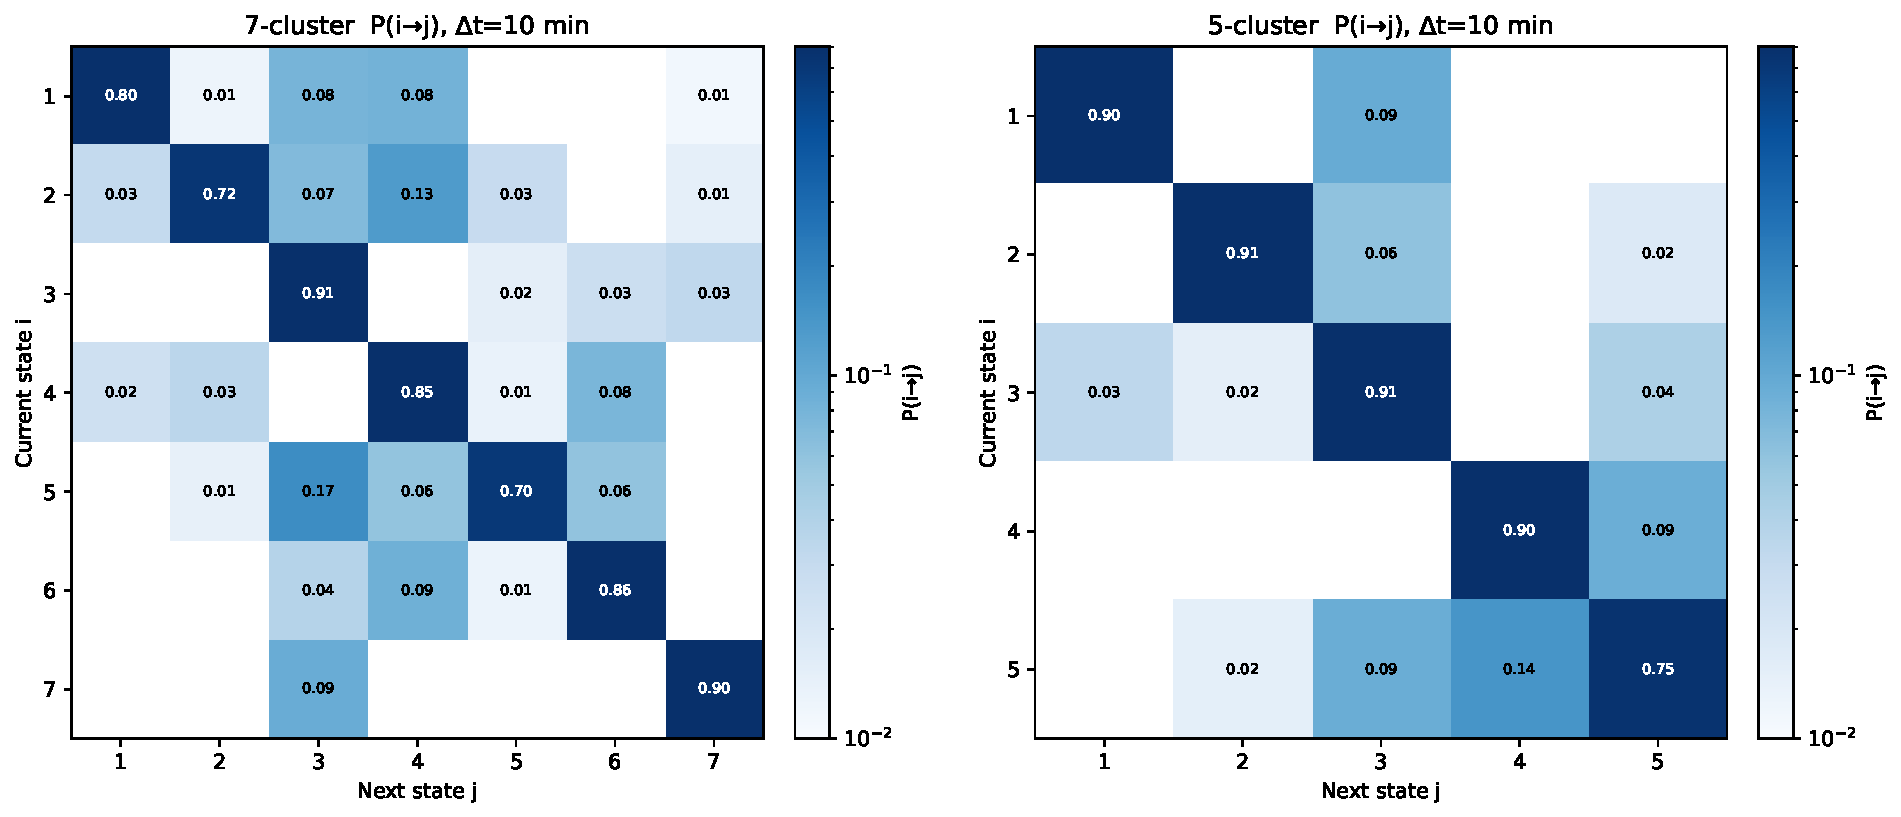
\includegraphics[width=0.78\textwidth]{fig2_transition_matrices.pdf}
\caption{Transition matrices $P(i\!\to\!j)$ at the 10-min chain step (log colour
scale, entries $<0.01$ masked). Both chains are strongly diagonal-dominant
(self-persistence $0.75$--$0.91$).}
\label{fig:T}
\end{figure}

Both transition matrices (Fig.~\ref{fig:T}) are strongly diagonal-dominant and
share the same off-diagonal topology: the organized and quiescent states exchange
among themselves and with the moist band, while the dry/active states form a
separate basin. The relaxation spectra are consistent: the slowest non-trivial
mode has $\tau_2 = 144$~min ($K=7$) vs.\ $173$~min ($K=5$), and both chains
produce a hierarchy of modes from $\sim$25~min to $\sim$3~h. Coarsening to 5
states does not collapse or invent slow timescales; it merges fast,
weakly-occupied transients (the $K=7$ chain has two extra modes near
$\tau\approx26$~min).

\section{Two-regime leading mode $v_2$}

\begin{figure}[htbp]
\centering
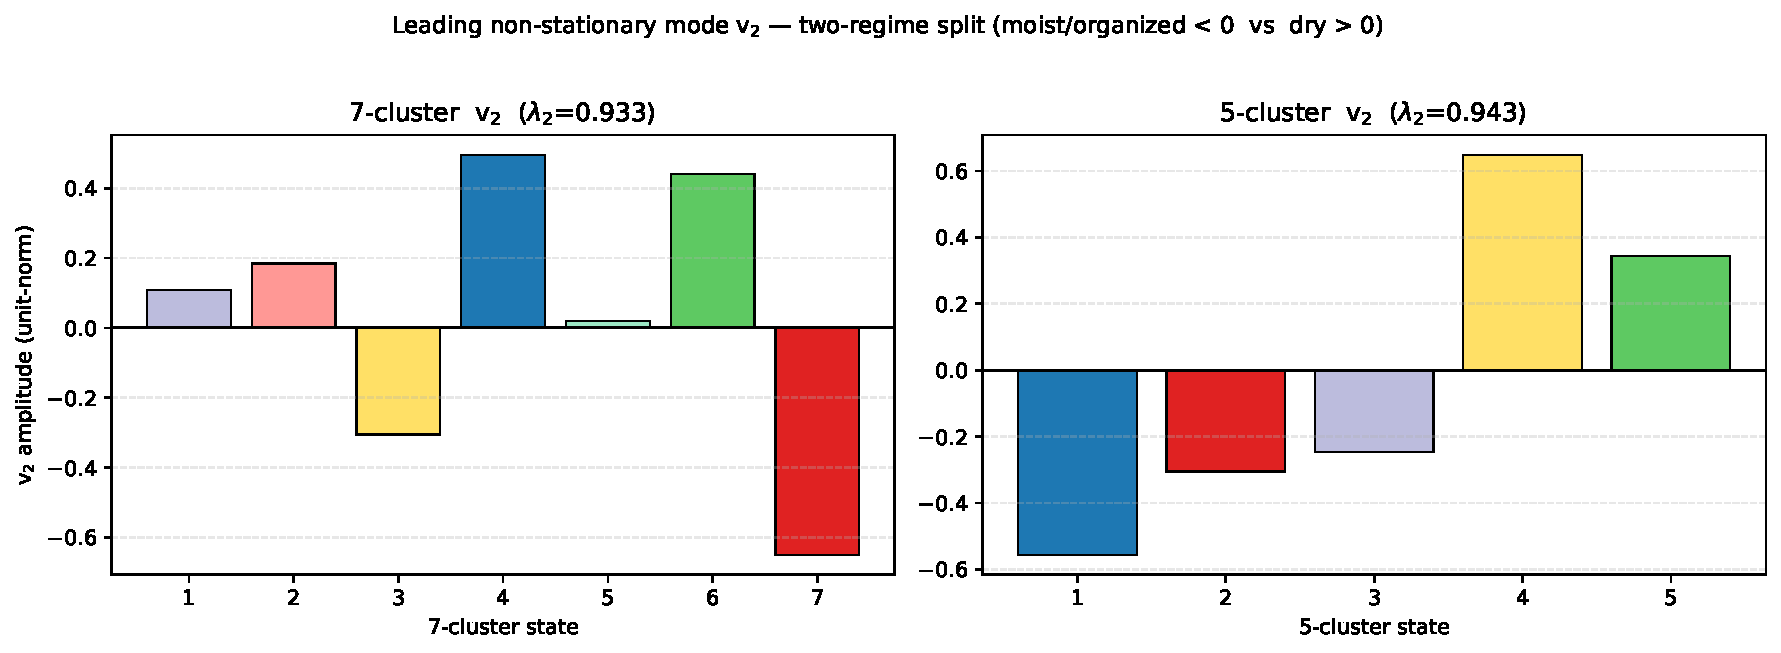
\includegraphics[width=0.6\textwidth]{fig3_v2.pdf}
\caption{Leading non-stationary right eigenvector $v_2$ (plain unit-norm
amplitudes; the arbitrary sign is fixed so the organized cluster is negative).
Both models show a clean two-regime split between the moist/organized side
($v_2<0$) and the dry side ($v_2>0$).}
\label{fig:v2}
\end{figure}

The two-regime structure survives (Fig.~\ref{fig:v2}). At $K=5$ the split is
sharp: $v_2<0$ for the moist/organized group $\{1,2,3\}$ and $v_2>0$ for the dry
group $\{4,5\}$, i.e.\ the slowest mode is a moisture/organization see-saw. At
$K=7$ the same contrast dominates---the largest amplitudes are the organized
7c\,7 ($-0.65$) and quiescent 7c\,3 ($-0.31$) against the dry/active 7c\,4
($+0.50$) and 7c\,6 ($+0.44$)---but the extra weakly-occupied states (7c\,1,
7c\,2, 7c\,5) carry small, mixed-sign amplitudes that blur the partition. The
five-state model expresses the same physical mode more cleanly.

\section{Markovianity of the organized cluster}

\begin{figure}[htbp]
\centering
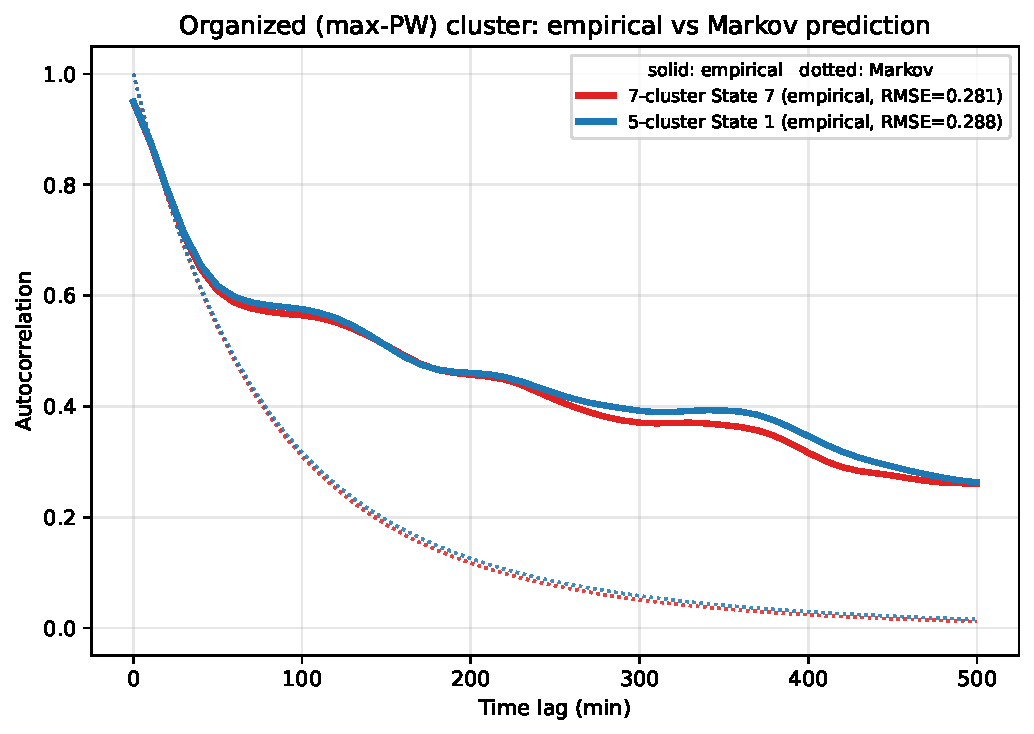
\includegraphics[width=0.42\textwidth]{fig4_markovianity.pdf}
\caption{Indicator autocorrelation of the organized (max-PW) cluster: empirical
(solid) vs.\ Markov-chain prediction (dotted), for both models. In both cases the
empirical curve persists far above the Markov prediction, signalling residual
non-Markovian memory.}
\label{fig:mk}
\end{figure}

The organized cluster is markedly non-Markovian in both models, and to nearly the
same degree (Fig.~\ref{fig:mk}): the autocorrelation--Markov RMSE is $0.275$ for
7c\,7 and $0.287$ for 5c\,1, with almost identical curves that stay near $0.25$ at
500~min while the Markov prediction has decayed to zero. The most Markovian cluster
in both models is the large quiescent core (RMSE $0.078$/$0.087$). The one
substantive difference is the \emph{second} memory-carrying regime: at $K=7$ it is
a distinct state, 7c\,6 (high PC2, RMSE $0.254$), whereas at $K=5$ that memory is
absorbed into 5c\,4 (RMSE $0.227$, fed by 7c\,4 and 7c\,6 per the mapping). The
five-state model retains the strongest non-Markovian signal cleanly but partially
merges the two organized memory regimes that $K=7$ keeps separate.

\section{Conclusion: 5 or 7 clusters?}

\textbf{All four headline results are robust to cluster count}---the
precipitation/organization plane, the organized high-PW cluster, the two-regime
$v_2$ mode, and the non-Markovianity of the organized cluster all appear, with
quantitatively similar values, at both $K=5$ and $K=7$. None of the paper's
qualitative conclusions is an artifact of choosing seven states. \textbf{Five
clusters is the parsimonious choice}: it preserves the two extreme states almost
verbatim (organized 7c\,7\,$\equiv$\,5c\,1, quiescent 7c\,3\,$\equiv$\,5c\,3),
gives a slightly cleaner $v_2$ split and a marginally stronger PC2--PW
correlation, and merges only weakly-occupied, fast-relaxing transients.
\textbf{Seven clusters earns its extra states} in one respect that matters here:
it resolves the active/organized lobe into \emph{two} distinct non-Markovian
regimes (7c\,6 and 7c\,7) that $K=5$ partially merges into 5c\,4 and 5c\,1.



\end{document}
